\chapter{Task 18: Turing Patterns}

\section{Task Description}
The goal of this task is to analyze a Turing activator-inhibitor dynamics on networks, with specific suggestion to replicate the findings of \cite{main_network}. 
\noindent
A system governed by a reaction-diffusion mechanism can exibit pattern emergence when perturbed from an initial linearly stable equilibrium state. The conditions for pattern initiation are found through linear stability analysis. The subsequent evolution of the pattern is non-linear and eventually results in a steady state (that can be either stationary or time dependent).
\\
\textbf{A note:} The authors of \cite{main_network} only state the conditions that must hold for pattern formation on the network. In fact, they can be derived with only a few minor changes in the same way as one does for pattern formation in a continuous medium. However, if the reader is not familiar with the traditional Turing patterns in continuous space (like me before this work), those relations are not at all evident. I wanted to get a true understanding of what I was going to simulate. That is why I studied in detail the case of the continuous medium and then I derived the conditions stated by the authors of \cite{main_network}. However, this meant that, to keep the workload manageable, I was able to focus only on the analysis of the \textbf{pattern initiation} stage and disregard the anaylis of the multistability and histeresis effects done in the second part of the article.

\section{Mathematical Model}
\subsection{Definitions}
A network-organized activator-inhibitor system can be defined in very close analogy to what one does for continuous media. 
In the network case, equations for the system are:
$$
\begin{cases}
\dot{u}_i(t) = f(u_i\, v_i) - \epsilon\,[L\,u(t)]_i \\
\dot{v}_i(t) = g(u_i\, v_i) - \epsilon\, \sigma [L\,v(t)]_i \\
\end{cases}
$$
Here, $\mathbf{u} = (u_1, \cdots u_N)$ and $\mathbf{v} = (v_1, \cdots v_N)$ are, respectively, the concentrations of the activator substance and the inhibitor substance on the $N$ nodes of the network. The reactions take place locally, on each node, and are encoded in the reaction terms $f(u_i\, v_i)$ and $f(u_i\, v_i)$. L is the laplacian matrix, defined as $L=D-A$. The diffusivity of the activator species is $\epsilon$, while that of the inhibitor is $\epsilon\,\sigma$, so that $\sigma$ is the ratio between them.

So far, the above are just the general equations of a reaction-diffusion system. In order to have a Turing mechanism, the reaction term need to satisfy the following basic requirements:
\begin{enumerate}
	\item Existence of a homogeneous equilibrium $(\overline{u},\, \overline{v})$ which is linearly stable in absence of diffusion (indeed, the key idea of the Turing model is that the instability is driven by diffusion, and appears only above a certain threshold function of the diffusion parameters) :
		$$
		\centering
		\begin{pmatrix}
			u_i(t) \\
			v_i(t)
		\end{pmatrix} \equiv  
		\begin{pmatrix}
			\overline{u} \\
			\overline{v}
		\end{pmatrix}
        \quad \forall i 
		\quad \text{where} \quad f(\overline{u}\,, \overline{v}) = g(\overline{u}\,, \overline{v})=0 \quad \text{and, given that}
		$$
		$$
		 \quad J(\overline{u}\,, \overline{v}) := 
		\begin{pmatrix}
 			f_u & f_v \\
 			g_u & g_v
 		\end{pmatrix}, \quad
 		\begin{cases}
 			\text{tr}(J)= f_u + g_v < 0\\
 			\text{det}(J) = f_u\cdot g_v f_v\cdot g_u>0
 		\end{cases}
		\text{(see \ref{app:bifurcation_diagram})}
		$$
	\item Correct qualitative behaviour of reactions in the neighborhood of the fixed point $(\overline{u},\, \overline{v})$: \newline
    the activator $u$ is supposed to enhance its own production and the production of the inhibitor $v$. Viceversa, the inhibitor $v$ is supposed to suppress the production of both the activator $u$ and itself. The functions $f,\, v$ need to reflect this behaviour, at least in a neighbourhood of the equilibrium $(\overline{u},\, \overline{v})$. Mathematically:
    \begin{center}
    \begin{minipage}{0.4\textwidth}
    \centering
    $$
           \begin{cases}
         f_u > 0,\quad f_v < 0 \\
         g_u >0,\quad  g_v <0 \\      
        \end{cases} 
    $$
    \end{minipage}
    \begin{minipage}{0.5 \textwidth}
    \centering
	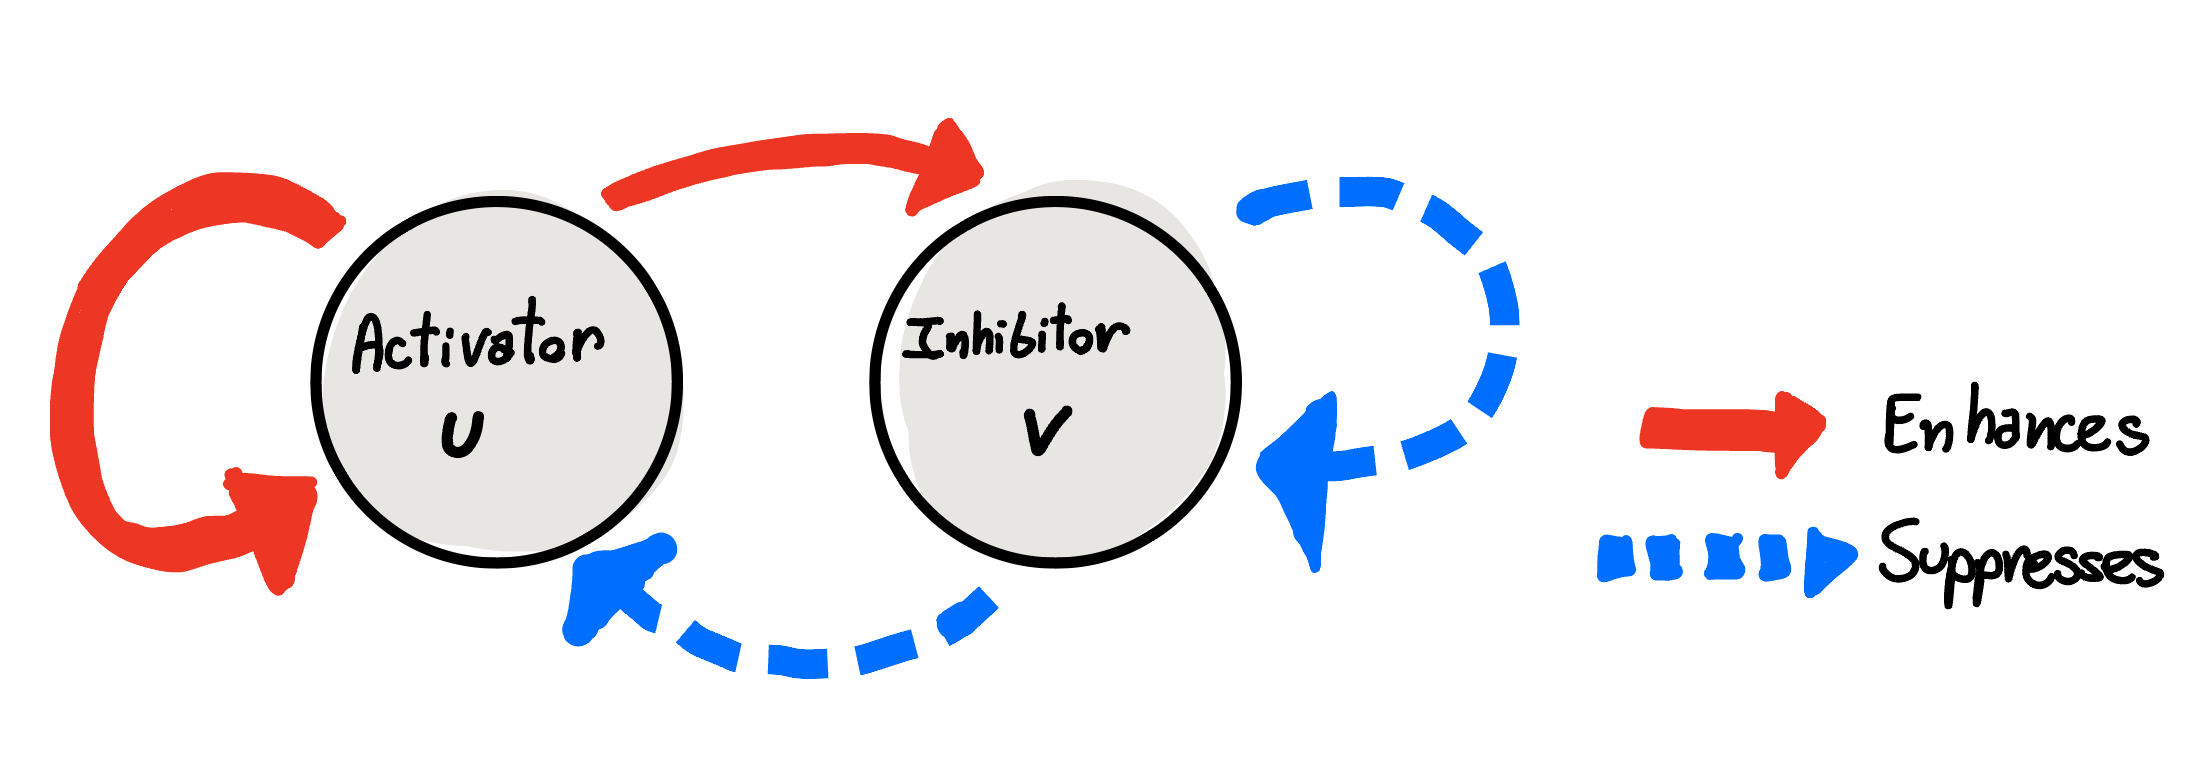
\includegraphics[width=0.9\textwidth]{images/turing/diagram.jpeg}
 \label{fig:diagram}
    \end{minipage}
    \end{center}
\end{enumerate}
These requirements are just the same as in the case for the continuous medium. 
\subsection{Conditions for diffusion-driven instability}
Diffusion driven instability is investigated by means of linear stability analysis. A small random perturbation $\delta\,u_i,\, \delta\,v_i$ is added at each node, starting from the homogeneous equilibrium state. A linearized system of equations is obtained for the evolution of the perturbation:
\begin{equation}
    \begin{cases}
    u_i(t) = \overline{u} + \delta\, u_i(t)\\
    v_i(t) = \overline{v} + \delta\, v_i(t)
    \end{cases}
    \rightarrow 
    \begin{cases}
    \delta\, \dot{u}_i(t) \simeq \quad     f_u\, \delta u_i(t) +  f_v\, \delta v_i(t) - \epsilon\,[L\cdot (\overline{u}+ \delta u(t))]_i\\
    \delta\, \dot{v}_i(t) \simeq \quad 
    g_u \, \delta u_i(t) +  g_v \, \delta v_i(t) - \epsilon\,\sigma\,[L(\overline{v}+ \delta v(t))]_i
    \end{cases}
\end{equation}
But $L\,\overline{u} = L\,\overline{v} = 0$, since the constant vectors $u$ and $v$ are eigenvectors of the laplacian with eigenvalue zero.
In the case of a continuous medium, the perturbation is expanded as a Fourier series of plane waves. The rationale of this is that it makes the PDE turn into an eigenvalue problem.
In the network case, we instead write the perturbation as:
\begin{equation*}
    \begin{pmatrix}
    \delta u_i (t) \\
    \delta v_i (t) \\
    \end{pmatrix}
    =
    \begin{pmatrix}
        1 \\
        B_n \\
    \end{pmatrix}
    \cdot \sum_{n=1}^{N}\, c_n\,\Phi_i^{(n)}\, e^{\lambda_n\,t} \\
\end{equation*}
Where $\Phi^{(n)}$ is the $n-th$ eigenvector of the laplacian matrix $L$ and its corresponding eigenvalue is $\Lambda_n$ ($0=\Lambda_1 \leq \Lambda_2 \leq \cdots \Lambda_N$). The coefficients $\{c_n\}$ are determined by the initial conditions $(t=0)$. By doing this, the system of equations is turned into a $\Lambda -$dependent eigenvalue problem. In fact, if we plug the ansaltz 
\begin{equation*}
    \begin{pmatrix}
    \delta u_i (t) \\
    \delta v_i (t) \\
    \end{pmatrix}
    =
    \begin{pmatrix}
        1 \\
        B_n \\
    \end{pmatrix}
    \cdot  c_n\,\Phi_i^{(n)}\, e^{\lambda_n\,t} \\
\end{equation*}
into the linearized system of equations, we get:
\begin{equation*}
    \begin{pmatrix}
        \delta \dot{u}_i \\
        \delta \dot{v}_i \\
    \end{pmatrix}
    =
    \begin{pmatrix}
        f_u - \epsilon\,\Lambda_n & f_v \\
        g_u & g_v -\epsilon\,\sigma\,\Lambda_n \\
    \end{pmatrix}
    \cdot 
        \begin{pmatrix}
        \delta u_i \\
        \delta v_i \\
    \end{pmatrix}
\end{equation*}
\begin{equation*}
    \rightarrow
        \lambda_n \cdot
        \begin{pmatrix}
        1 \\
        B_n\\
    \end{pmatrix}
    =
    \begin{pmatrix}
        f_u - \epsilon\,\Lambda_n & f_v \\
        g_u & g_v -\epsilon\,\sigma\,\Lambda_n \\
    \end{pmatrix}
    \cdot 
        \begin{pmatrix}
        1 \\
        B_n\\
    \end{pmatrix}
\end{equation*}
Or, in compact form:
\begin{equation*}
    \lambda_n\, \mathbf{v}_n = M(\Lambda_n,\,\sigma,\,\epsilon)\, \mathbf{v}_n
\end{equation*}
The differences between the network case and the continuous medium case end here. From now on, the steps are exactly the same. We are looking for instability, thus we want to find the range of parameters $(\sigma,\, \epsilon)$ that produce $\mathcal{R}e\{\lambda_{\pm}(\Lambda)\}>0$ for a positive range of $\Lambda$'s. \\
First, we must have that at least one of the following holds
\begin{equation*}
    \begin{cases}
        \text{det}[M(\Lambda,\,\sigma,\,\epsilon)]<0 \\
        \text{tr}[M(\Lambda,\,\sigma,\,\epsilon)]> 0 \\
    \end{cases}
\end{equation*}
But $\text{tr}[M(\Lambda,\,\sigma,\,\epsilon)] = \text{tr}[J] - \epsilon\, \Lambda\, (1+\sigma)<0$ because the homogeneous state is a stable equilibrium, then the only possibility is that $\text{det}[M(\Lambda,\,\sigma,\,\epsilon)]< 0$. \\
Some quick boring algebra now:
\begin{equation*}
    \text{det}[M(\Lambda,\,\sigma,\,\epsilon)] = \epsilon^2\,\sigma\,\Lambda^4 - \epsilon\,(g_v +\sigma\,f_u) \Lambda + \text{det}[J] \overset{!}{\leq} 0 \quad \text{for some}\, \Lambda >0
\end{equation*}
\begin{minipage}{0.6\textwidth}
This is a parable of kind $y = a\,x^2 - b\,x + c$ with  $(a,\,b,\,c>0)$, so the minimum is reached at coordinates $(x_{min},\,y_{min}) = (\frac{b}{2\,a}\,, c-\frac{b^2}{4\,a})$. The parable touches the $x$ axis ($y_{min}\leq 0$) $\iff$ $\Delta^2 = b^2-4\,a\,c \geq 0$.
\end{minipage}
\hfill
\begin{minipage}{0.38\textwidth}
    \centering
    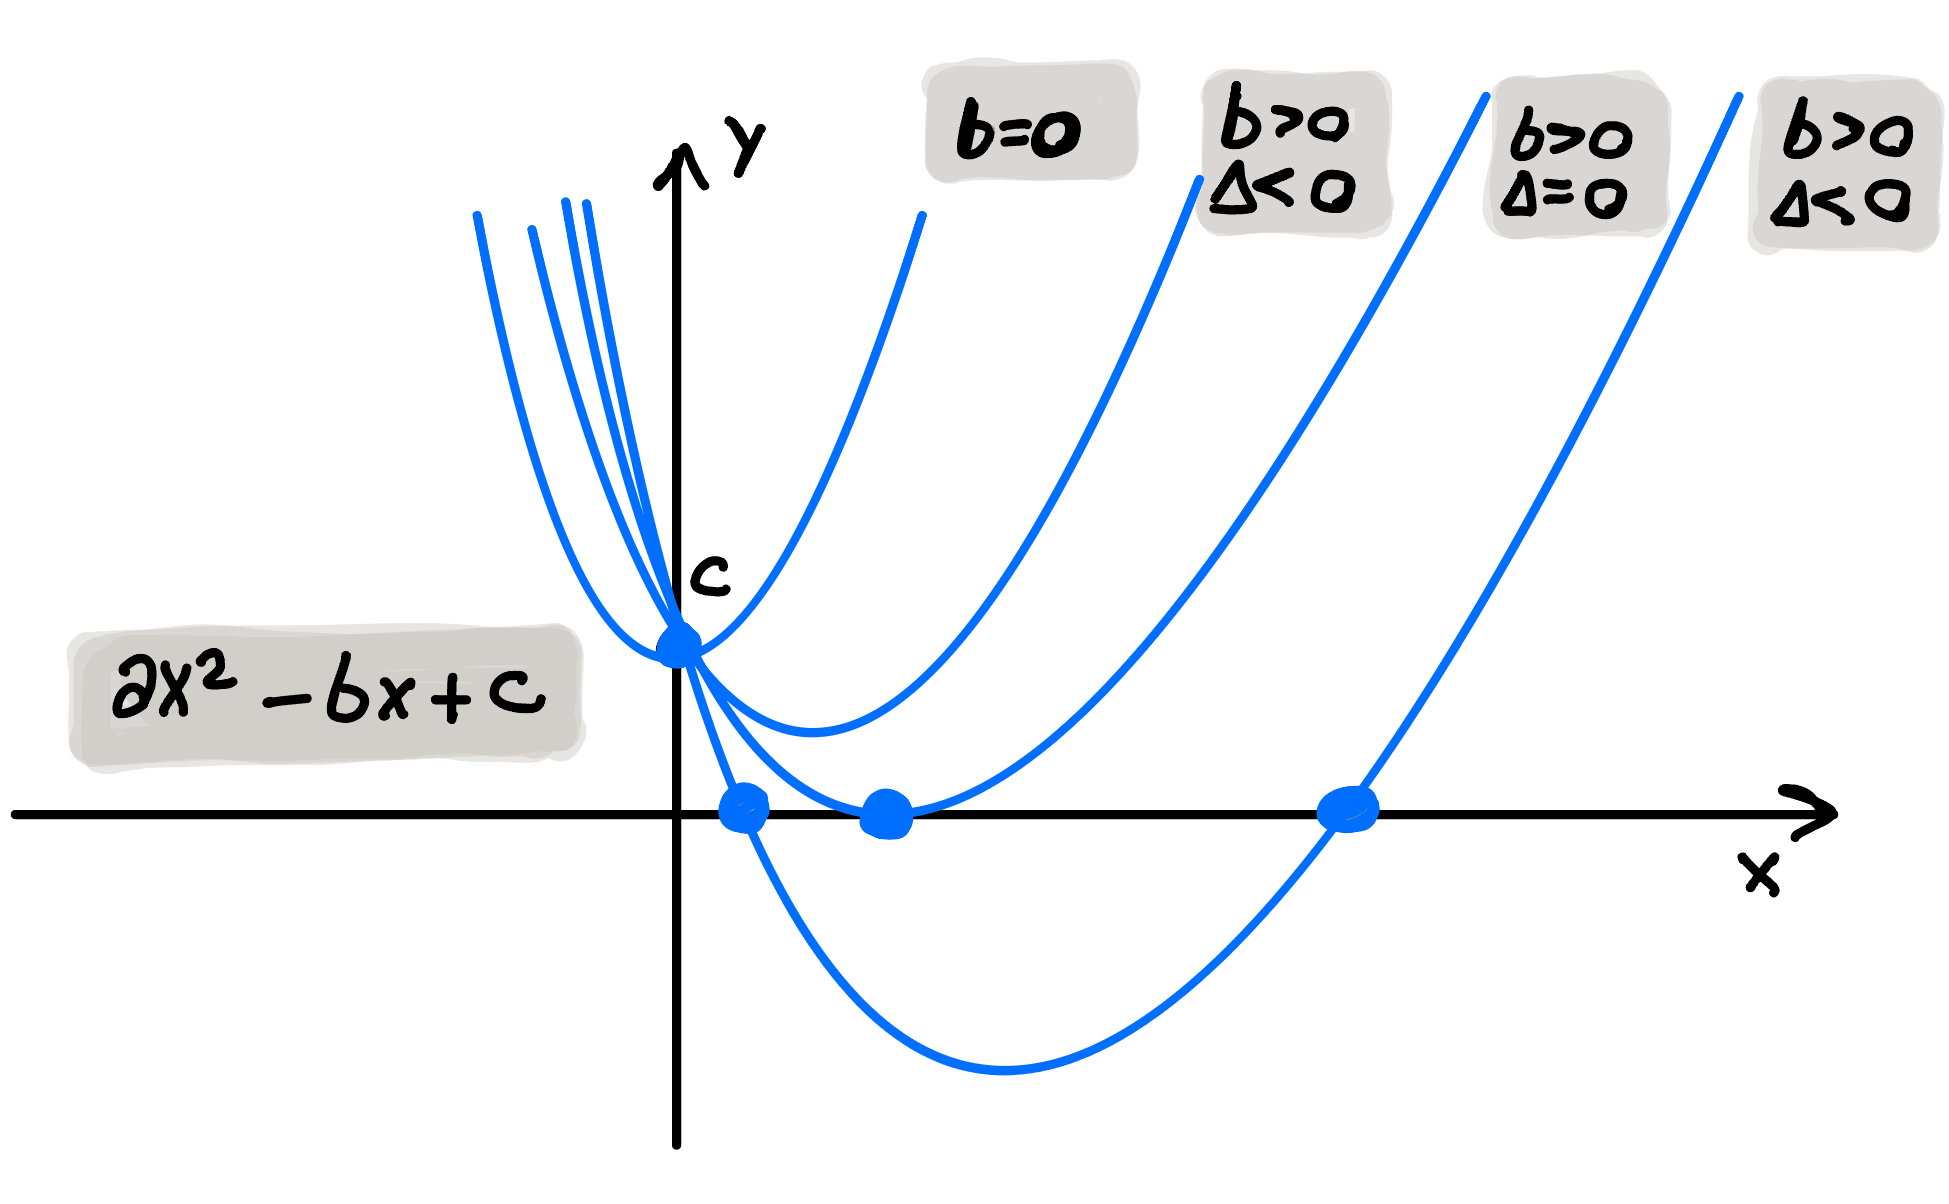
\includegraphics[width=\textwidth]{latex_source/images/turing/parable.jpeg}
\end{minipage}
\newline
We require:
\begin{equation*}
    \begin{cases}
        x_{min}(\epsilon,\,\sigma)>0 \\
        y_{min}(\epsilon,\,\sigma)\leq 0 \\
    \end{cases}
    \quad
        \begin{cases}
        \epsilon\,(g_v +\sigma\,f_u) > 0 \\
        [\epsilon\,(g_v +\sigma\,f_u)]^2 \geq 4\,\epsilon^2\,\sigma\,\text{det}[J] \\
    \end{cases}
\end{equation*} 
From the first one, we notice that there exists a minimum value threshold for $\sigma > \sigma_{min}= \frac{|g_v|}{f_u}$. Also, since $\text{tr}\,[J]=(-|g_v| +f_u)<0$, then $\sigma_{min}> 1$: a necessary (but still not sufficient) condition for pattern initiation is that the inhibitor diffuses faster than the activator.
\begin{equation*}
    \begin{cases}
        \sigma > \sigma_{min} >1  \\
        f_u^2\,\sigma^2 + 2\,(f_u\,g_v-2\,\text{det}[J])\,\sigma + g_v^2 \geq 0 
    \end{cases}
    \quad 
    \begin{cases}
    \sigma > \sigma_{min} >1  \\
    \sigma < \sigma_{-}(<\sigma_{min}) \quad \text{or} \quad  \sigma > \sigma_{+}\\
    \end{cases}
\end{equation*} 
Where $\sigma_{\pm}$ are the roots of the quadratic equation:
\begin{equation*}
    \sigma_{\pm} = \frac{(f_u\,g_v - 2\,f_v\,g_u)\,\pm 2\,\sqrt{f_v\,g_u\,(f_v\,g_u-f_u\,g_v))}}{f_u^2}
\end{equation*}
The function $y_{min}(\sigma)$ reaches its maximum for $\sigma=\sigma_{min}$ and goes to $-\infty$ for both $\sigma\rightarrow0^{+}$ and $\sigma\rightarrow +\infty$. Also, the lower-branch root $\sigma_{-}$ is below the threshold value $\sigma_{min}$. Then, both our requirements are satisfied if and only if $\sigma>\sigma_{+}$. In summary, the necessary and sufficient condition for instability is
\begin{equation*}
 \sigma > \sigma_c :=  \frac{(f_u\,g_v - 2\,f_v\,g_u)\, + 2\,\sqrt{f_v\,g_u\,(f_v\,g_u-f_u\,g_v))}}{f_u^2}
\end{equation*}
\textbf{Critical eigenvalue and graph finite size effect} \newline
The critical eigenvalue $\Lambda$ is determined for give $\epsilon$:
\begin{equation}
\label{eq:critical_eigenvalue}
    \Lambda_c(\epsilon) := \Lambda(\sigma=\sigma_c,\,\epsilon) = \frac{g_v + \sigma_c\,f_u}{2\,\epsilon \,\sigma_c} = (\cdots) = \frac{1}{\epsilon}\,\sqrt{\frac{\text{det}[J]}{\sigma_c}}
\end{equation}
For $\sigma$ above the critical threshold, a finite range [$\Lambda_1\,\Lambda_2$] centered around $\Lambda_c$ appears where the corresponding mode is unstable. However, the eigenvalue spectrum of the laplacian matrix is not continuous. Instability will appear if there are allowed modes that fall inside this range.
In particular, the eigenvalue spectrum of the laplacian is bounded above for a graph of finite size. If the mobility $\epsilon$ is small enough, the critical eigenvalue could lay beyond the largest eigenvalue of the graph, and instability would not occur.
This finite-size effect appears also in the case of a continuous medium. There, instability cannot occur when the spatial domain is too small and the largest allowed wavelength is less than the critical wavelength.
\medskip \newline
\textbf{Dispersion relation $\lambda(\Lambda;\, \sigma,\,\epsilon)$} \newline
Finally, the growing rate of the unstable mode, $\lambda_n = \lambda(\Lambda_n)$ is calculated from the caractheristic polynomial of $M(\Lambda_n, \sigma,\,\epsilon)$:
\begin{equation*}
    p(\lambda) = (\lambda-\lambda_1)\cdot(\lambda-\lambda_2) = \lambda^2 - \text{tr}[M(\Lambda,\,\sigma,\,\epsilon)]\cdot \lambda + \text{det}[M(\Lambda,\,\sigma,\,\epsilon)]
\end{equation*}
\begin{align*}
    \lambda_{\pm} &=\frac{1}{2}\,\left[\text{tr}[M]\pm \sqrt{\text{tr}[M]^2-4\,\text{det}[M]}\right] = \frac{1}{2}\,\left[-|\text{tr}[M]|\pm \sqrt{\text{tr}[M]^2-4\,\text{det}[M]}\right] \\
    &= \frac{1}{2}\, \left[\left[f_u + g_v - (1+\sigma)\,\epsilon\,\Lambda\right] + \sqrt{4\,f_v\,g_u + \left[f_u - g_v -(1-\sigma)\,\epsilon\,\Lambda\right]^2}\right]
\end{align*}
In the instability region, $\text{tr}[M] <0$ and $\text{det}[M]<0$, then eigenvalues are real and distinct. Also, the lower branch is always negative so we are not interested in it. By comparison with the graph of $\text{det}[M(\Lambda,\,;\epsilon,\,\sigma]$, we get the qualitative dependence of $\lambda$ from $\Lambda$, commonly called "dispersion relation".
\newpage
\section{Numerical Simulations}
As in \cite{main_network}, the reaction terms are set as
\begin{equation}
    \begin{cases}
        f(u,v) = [\frac{a + b\,u -u^2}{c} - v]\, u \\
        g(u, v) = [u - (1+ d\,v)]\cdot v 
    \end{cases}
\label{eq:chosen_kinetics}
\end{equation}
with parameters $a\,=\,35,\, b=16,\, c= 9,\, d= 2/5$, 
helding a linearly stable fixed point $(\overline{u},\, \overline{v}) = (5, 10)$ and a critical diffusion ratio $\sigma_c \simeq 15.5$. \newline \noindent
\begin{figure}[H]
    \centering
    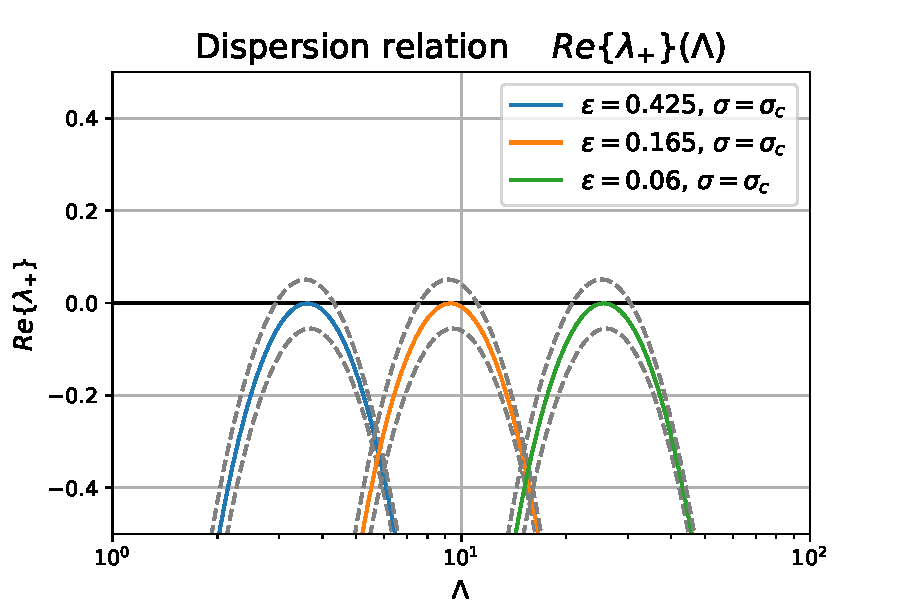
\includegraphics[width=0.8\textwidth]{latex_source/images/turing/multiple_dispersion.pdf}
    \caption{Dispersion relation for the chosen reaction kinetics [Eq. $\ref{eq:chosen_kinetics}$], at different values of the activator diffusivity $\epsilon$. The dashed grey lines are the dispersion curves slightly above and below the critical diffusivity ratio $\sigma_c$. As stated in [Eq. \ref{eq:critical_eigenvalue}], the critical eigenvalue $\Lambda_c$ is inversely proportional to the activator diffusivity $\epsilon$.}
\end{figure}
Following the choice of the authors, I simulated the dynamics on Barabasi-Albert scale free networks. I chose parameters $N = 200$ for the number of nodes and $\<k\> = 10$ for the mean degree. My activator diffusivity was $\epsilon = 0.12$, and my diffusivity ratio was $\sigma = 15.6 > \sigma_c = 15.5$. The reasoning for chosing a diffusivity ratio that is only slightly above the critical threshold is to keep the number of different allowed modes low.
\begin{figure}[H]
\subfigure[]{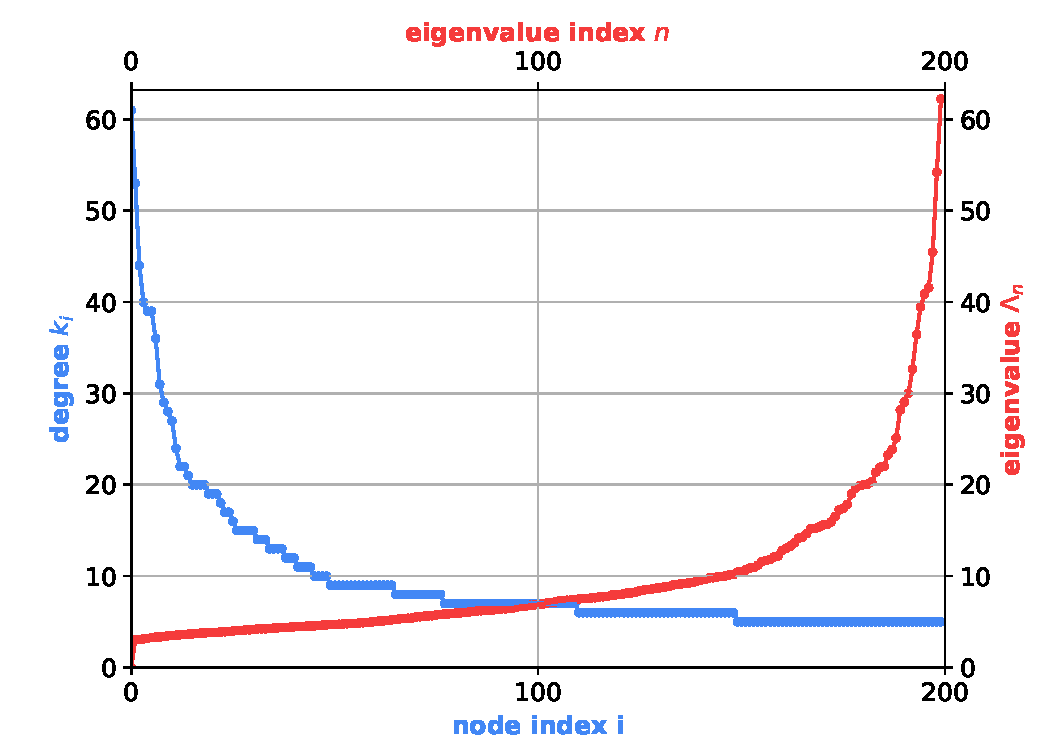
\includegraphics[width = 0.47\textwidth]{latex_source/images/turing/network_200.pdf}}
\subfigure[]{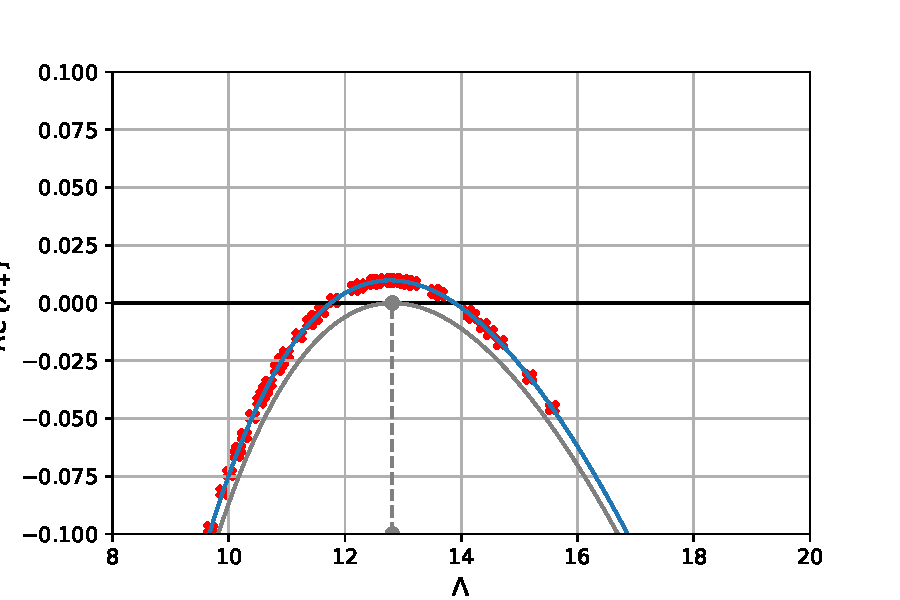
\includegraphics[width = 0.47\textwidth]{latex_source/images/turing/simulation_dispersion.pdf}}
\caption{Most relevant properties of the network used in the simulation. Subfigure (a) shows the degree spectrum and the laplacian eigenvalue spectrum of the chosen graph. Network nodes are indexed by decreasing degree. Subfigure (b) shows the dispersion relation curve. Critical eigenvalue is $\Lambda_c \simeq 12.8141$. The eigenvalue closest to $\Lambda_c$ is $\Lambda_n \simeq 12.64$, of index $n=157$. However, as one can see from the graph, the network eigenvalue spectrum comprehends several other allowed modes (red crosses) in the unstable range, and they are expected to contribute to pattern initiation as well.}
\end{figure}
\noindent
The initial homogeneous state $(\overline{u},\,\overline{v})$ was perturbed with a random uniform perturbation at each node of amplitude $0.05$. [Figure \ref{fig:snapshots}] show snapshots of the activator concentration on nodes at different times. Also, the GithHub repository \cite{git} contains a .mp4 video of the whole evolution. \medskip \newline \noindent
In the early stage, the pattern is expected to grow proportionally to the critical eigenvector, which is is the mode of largest growing rate: $\delta\,u(t),\, \delta\,v(t) \propto \Phi^{(n)}$.
In fact, when the initial uniform perturbation dies out and the pattern starts to grow, the activator substance distribution is located similarly to the critical eigenvector (see snapshot $t = 25.06$). Later on, the evolution becomes strongly non-linear and the pattern is reshaped (see snapshot at $t = 100.25$), till it settles into a stationary state (see snapshot at $t = 150.38$) where nodes are split into one activator-rich group and one activator-poor group. The authors found that this peculiar behaviour is well described in the framework of a mean field theory \cite{main_network}. \medskip \newline \noindent
An interesting thing one can notice in the initial stage pattern [Figure \ref{fig:snapshots}, snapshot at $t = 25.06$] is that the significant variations of the activator level are localized on a subset of nodes of close degree ($k \sim 25-75$). That is, only a specific subset of the network undergoes differentiation. This effect is was not a fortuity but is due to the fact that the laplacian eigenvectors in a large graph with a broad degree distribution tend to be localized around a specific degree $\overline{k}(\Lambda)$. Also, as authors report, a simple relation $\overline{k}(\Lambda) \simeq \Lambda$ seems to hold. I checked wether I could find the same behaviour for my graph (see [Figure \ref{fig:eigenvectors}] and [Figure \ref{fig:heatmap}].
\begin{figure}[H]
    \centering
    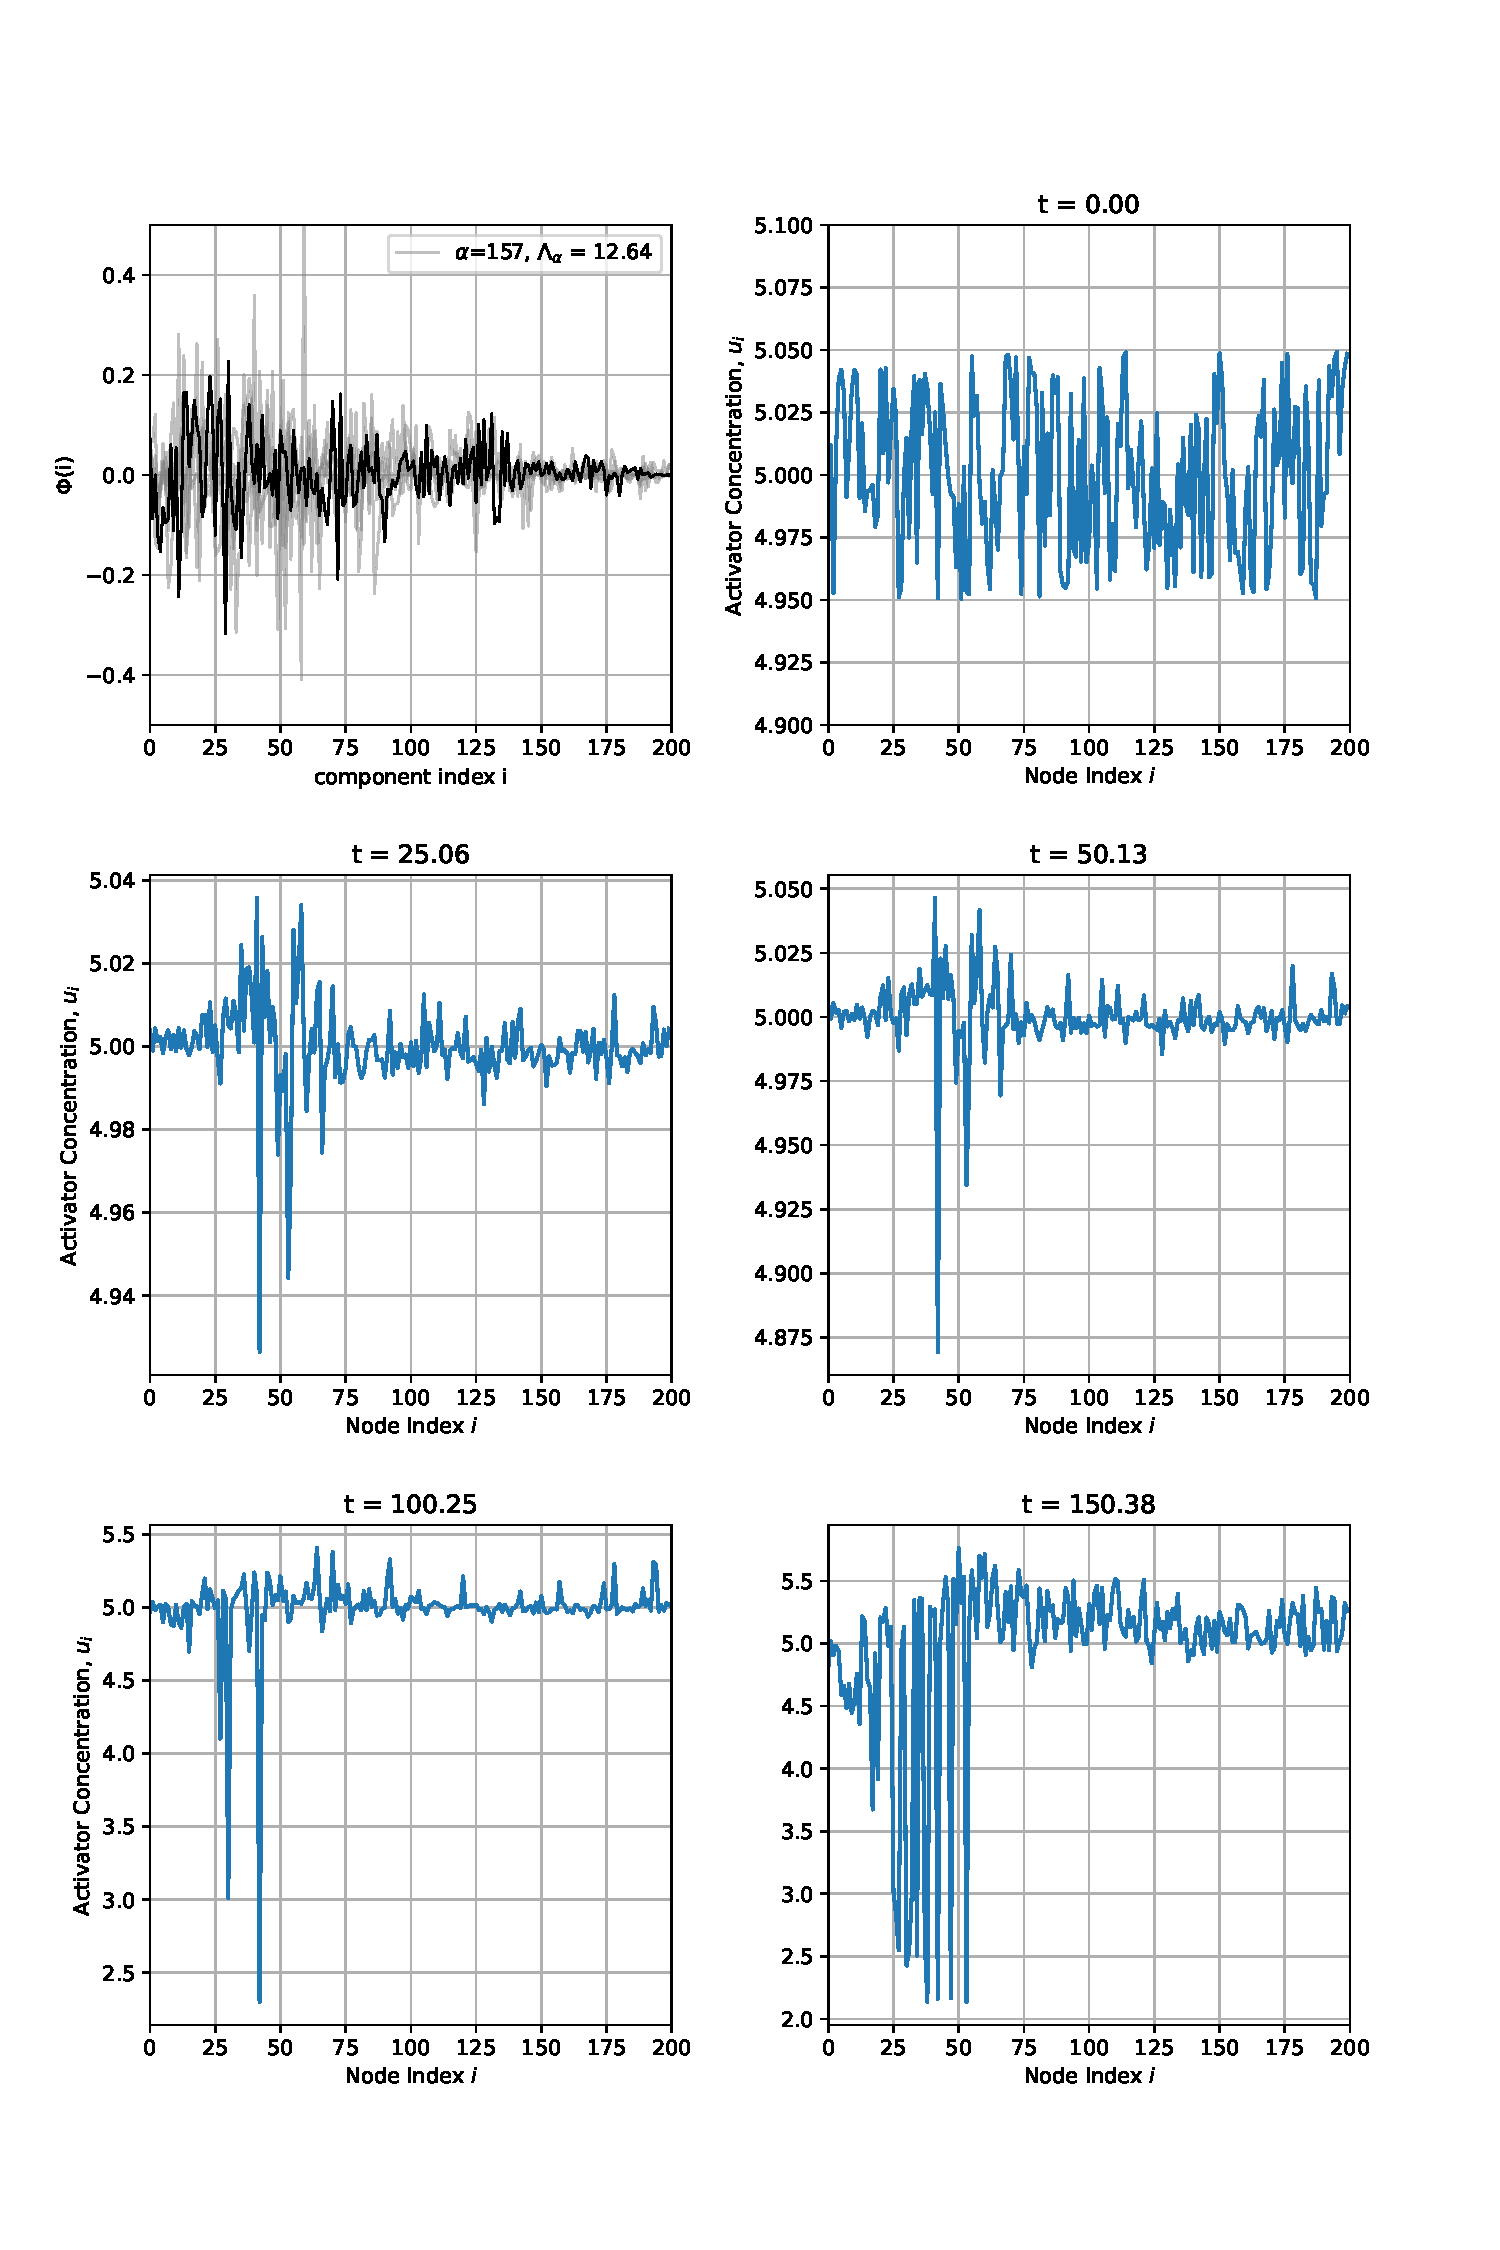
\includegraphics[width = 0.9\textwidth]{latex_source/images/turing/snapshots.pdf}
    \caption{Time evolution of the activator concentration. The subfigure at top left corner shows the components of the critical eigenvector (in black) and its closest neighbours in the unstable range (in grey).}
    \label{fig:snapshots}
\end{figure}
\begin{figure}[H]
\centering
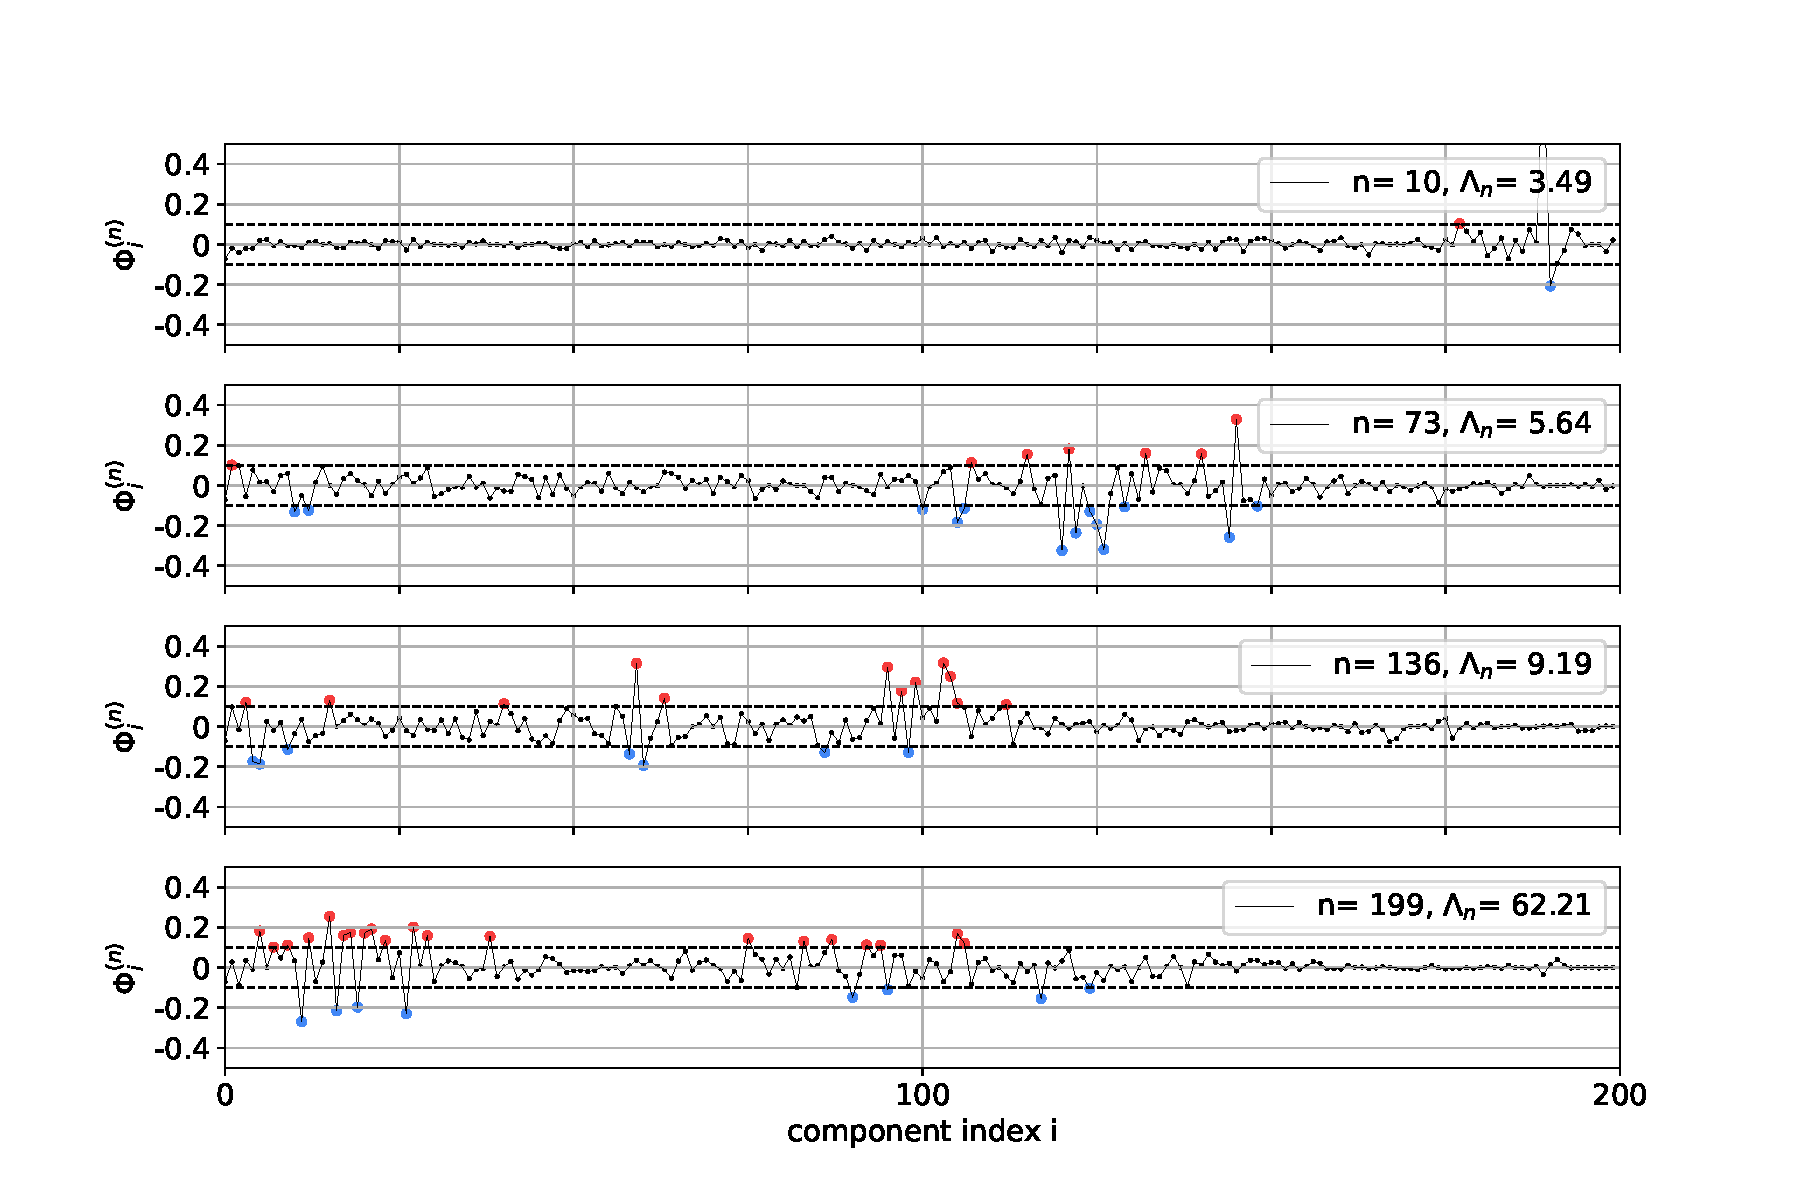
\includegraphics[width =\textwidth]{latex_source/images/turing/eigenvectors_200.pdf}
\caption{Localization of laplacian eigenvectors in 
a BA with $N=200$ and $\<k\> = 10$. Nodes nodes are ranked by their degree. With incrementing eigenvalue $\Lambda$, the characteristic degree becomes higher.}
\label{fig:eigenvectors}
\end{figure}

\begin{figure}[H]
    \centering
\subfigure[]{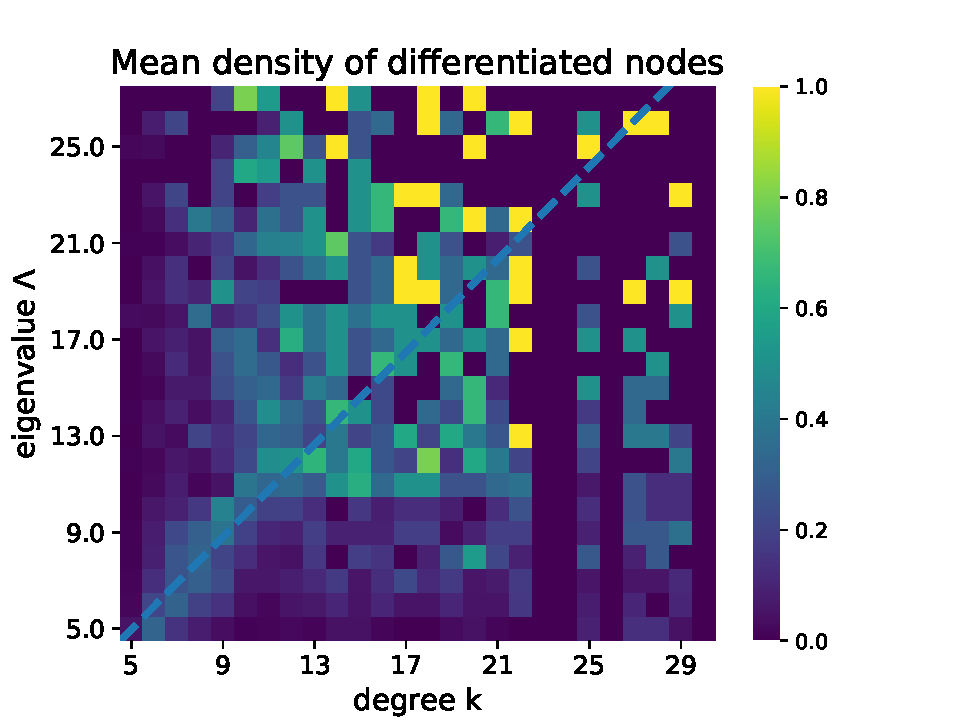
\includegraphics[width=0.48\textwidth]{latex_source/images/turing/density_200.pdf}}
\subfigure[]{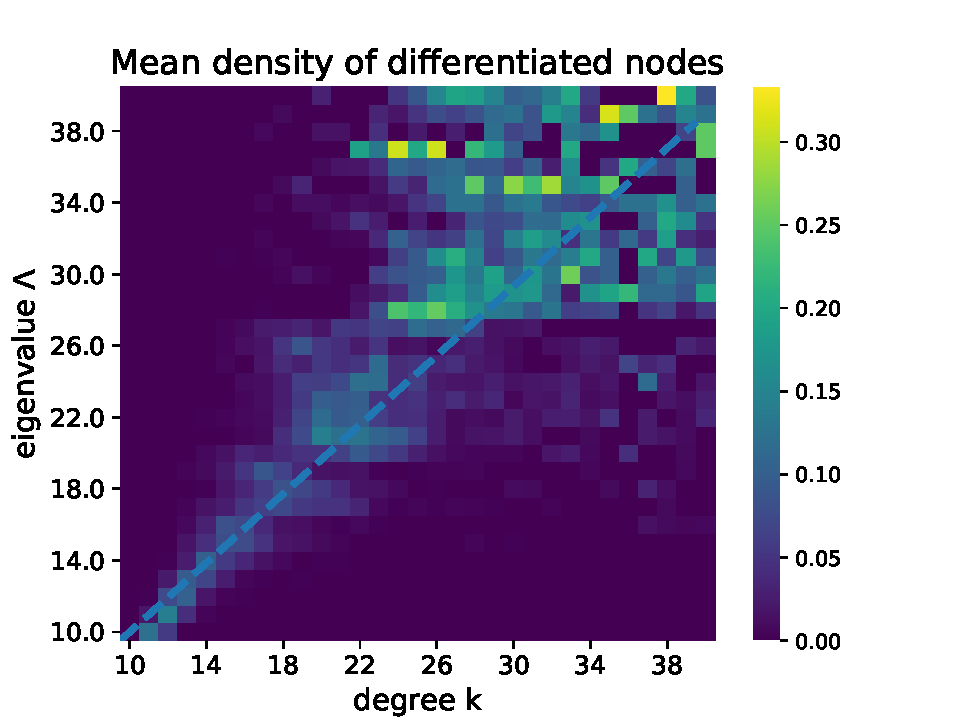
\includegraphics[width=0.48\textwidth]{latex_source/images/turing/density_1000.pdf}}
\caption{Localization of laplacian eigenvectors in a BA graph with $N=200$ nodes and $\<k\>=10$ (a) and in a BA graph with $N=1000$ nodes and $\<k\>=20$ (b). Eigenvalues have been grouped into bins of unitary width. The population of nodes inside each degree group, $N_k$, was calculated. The heatmap represents the mean density of differentiated nodes for each degree group $z = N_k^{\text{diff}}(\Lambda)/N_k$. A node $i$ of degree was considered to be differentiated with respect to eigenvalue $\Lambda_n$ if its eigenvector component satisfied, $|\Phi_i^{(n)}|> 0.1$. I found, like authors \cite{main_network} report, that approximately $\overline{k}(\Lambda) \propto \Lambda$ (dashed line) and that effect is more pronounced in the larger graph.}
\label{fig:heatmap}
\end{figure}

\nocite{bio_article}
\nocite{murray}
\nocite{altbook}
\newpage
\chapter*{Appendix}
\addcontentsline{toc}{section}{Appendix}
\textbf{Linear Stability of a 2x2 system}
\label{app:bifurcation_diagram}
 The linear stability requirement is satisfied if the jacobian matrix of $F(u,v) = (f(u,v), g(u,v))$ evaluated at the fixed point $(\overline{u}\,, \overline{v})$, $J_F(\overline{u},\, \overline{v})$, has all eigenvalues with negative real parts $\mathcal{R}e(\lambda_i)<0$. Say 
 \begin{equation*}
 		J_{F}(\overline{u}\,, \overline{v}) := \begin{pmatrix}
 			f_u & f_v \\
 			g_u & g_v
 		\end{pmatrix}
 \end{equation*}
Then
$$
Re\{\lambda_i\} <0 \iff 	J_{F}(\overline{u}\,, \overline{v})< 0\quad  \text{(neg. def.)} \iff \begin{cases}
		\text{tr}(J_F) < 0 \\
		\text{det}(J_F)>0
	\end{cases}
	\iff \begin{cases}
		f_u + g_v < 0 \\
		f_u\cdot g_v - f_v\cdot g_u>0
	\end{cases}
$$



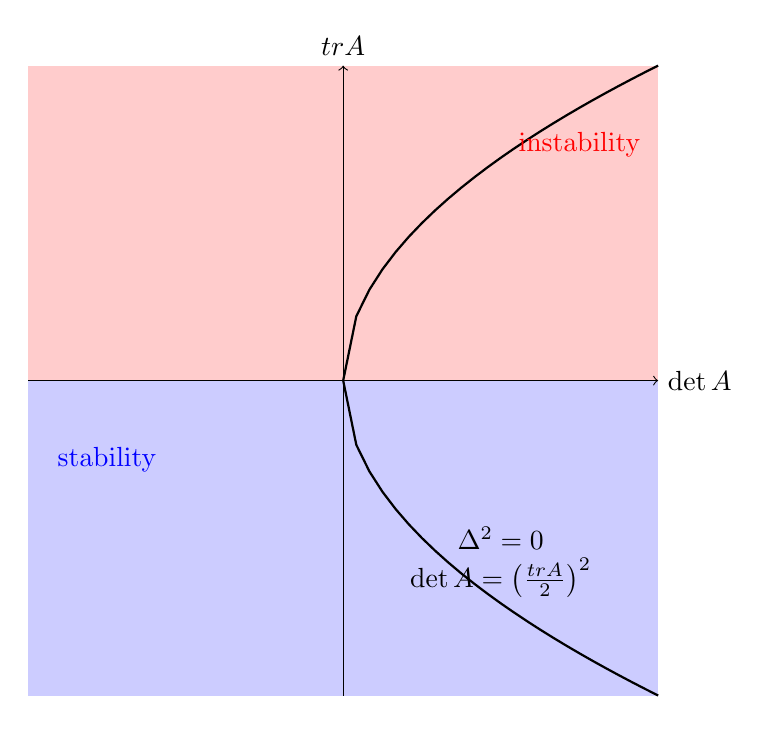
\begin{tikzpicture}
    % Set the size of the grid and the colors
    \fill[red!20] (-4,0) rectangle (4,4);
    \fill[blue!20] (-4,-4) rectangle (4,0);
    
    % Draw the axes
    \draw[->] (-4,0) -- (4,0) node[right] {$\det A$};
    \draw[->] (0,-4) -- (0,4) node[above] {$\operatorname{tr} A$};
    
    % Draw the parabola
    \draw[thick, domain=0:4] plot (\x, {sqrt(\x*4)}) node[right] {};
    \draw[thick, domain=0:4] plot (\x, {-sqrt(\x*4)}) node[right] {};
    
    % Stability and Instability regions
    \node[blue] at (-3,-1) {stability};
    \node[red] at (3,3) {instability};
    
    % Label for the critical point
    \node at (2, -2) {$\Delta^2=0$};
    \node at (2, -2.5) {$\det A = \left(\frac{\operatorname{tr} A}{2}\right)^2$};
\end{tikzpicture}
